\section*{Лабораторная работа}
\textbf{Содержание проекта:} Команда разработчиков из \textbf{16 человек} занимается созданием карты города на основе собственного модуля отображения. Проект должен быть завершен в течение \textbf{6 месяцев}. Бюджет проекта: 50 000 рублей.

На рисунке \ref{p0} показаны используемые ресурсы:
\begin{figure}[!h]
	\centering
	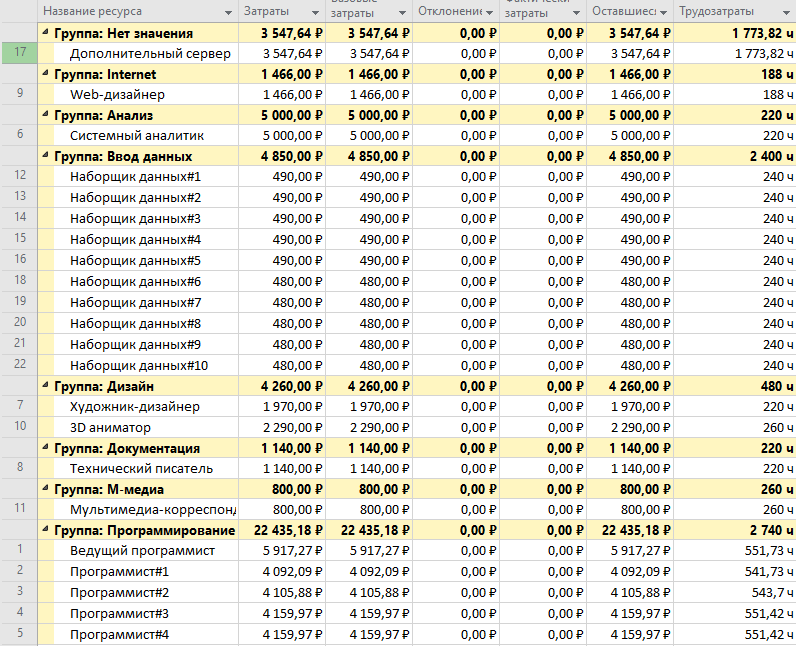
\includegraphics[width=1\linewidth]{inc/img/0.png}
	\caption{Используемые ресурсы}
	\label{p0}
\end{figure}

\newpage
\subsection*{Задание №1: Работа с таблицей освоенного объема}
На рисунке \ref{p1} изображена таблица освоенного объема:
\begin{figure}[!h]
	\centering
	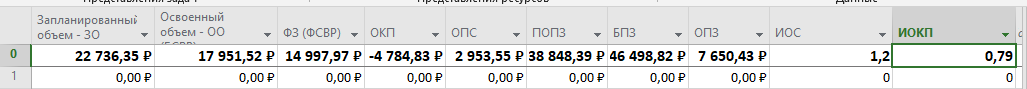
\includegraphics[width=1\linewidth]{inc/img/1.png}
	\caption{Таблица освоенного объема}
	\label{p1}
\end{figure}

По данному рисунку можно сделать следующие выводы, о показателях проекта:

\noindent ОКП < 0 => проект запаздывает

\noindent ОПС > 0 => проект находится в пределах сметы

\noindent ОПЗ < 0 => нет перерасхода средств

\noindent Затраты: 46 700,92 руб.

\noindent Длительность: 20,85 недель

\noindent Окончание: 01.08.23

\subsection*{Задание №2: Работа с отчетами проекта}


\section*{Выводы}


По итогу проделанной работы были получены навыки контроля за ходом реализации проекта возможностями программы Microsoft Project.